\documentclass[twocolumn,11pt]{abst}
\usepackage{url}
\usepackage{float}


% タイトル
\title{ロボコン用高出力モータドライバの開発}

\author{東出和賢(指導教員\,伊藤恒平$\cdot$林道大)}

%\urlstyle{rm}

\setcounter{page}{5}
\lhead{}
\chead{}
\rhead{{\sf 17・203}\\{\bf 機械工学科}}
\lfoot{}
%\cfoot{{\sf-\ M-\thepage \ -}}
\cfoot{
 \ifnum \value{page} < 10
  {\sf-\ M-0\thepage \ -}
 \else%
  {\sf-\ M-\thepage \ -}
 \fi%
}
\rfoot{}
\renewcommand{\headrulewidth}{3pt}
%\renewcommand{\footrulewidth}{1pt}



\begin{document}
%\layout
\maketitle
\thispagestyle{fancy}
\pagestyle{fancy}

\setlength{\baselineskip}{5.6truemm}
\kanjiskip=.07zw plus 3pt minus 3pt
\xkanjiskip=.07zw plus 3pt minus 3pt


% 本文

\section{はじめに}
\subsection{研究の背景}
当研究室では,高専ロボコンに出場するためのロボット設計,及び製作を行っており,
今年度のロボットは,高速な移動が必要であったので,高出力モータを使用した.
そこで,モータドライバに伊藤研究室で作成されたITOLAB MOTORDRIVERを使用した.
しかし,多くの不具合が発生し,目標とした移動速度を下回ってしまった.
また地区大会では,モータのトラブルが発生したが,原因は分からなかった.

以上のことから,当研究室のロボットが活躍するために,扱いやすい高出力モータードライバ
が有効だと考える.

\subsection{研究の目的}
ITOLAB MOTORDRIVERをもとに,当研究室で使用できる高出力
モータドライバの設計,作製を行う.

\section{ITOLAB MOTORDRIVER}
\subsection{ドライバの特徴}
ITOLAB MOTORDRIVERを図\ref{fig:driver}に示す.
ロボコンでは,ロボットに使用できる物品の上限価格が設定されている.また,ロボット
にフィードバック制御が必要であったので,
エンコーダが使用でき,製作コストが安いITOLAB MOTORDRIVERを使用することにした.
\begin{figure}[H]
  \begin{center}
    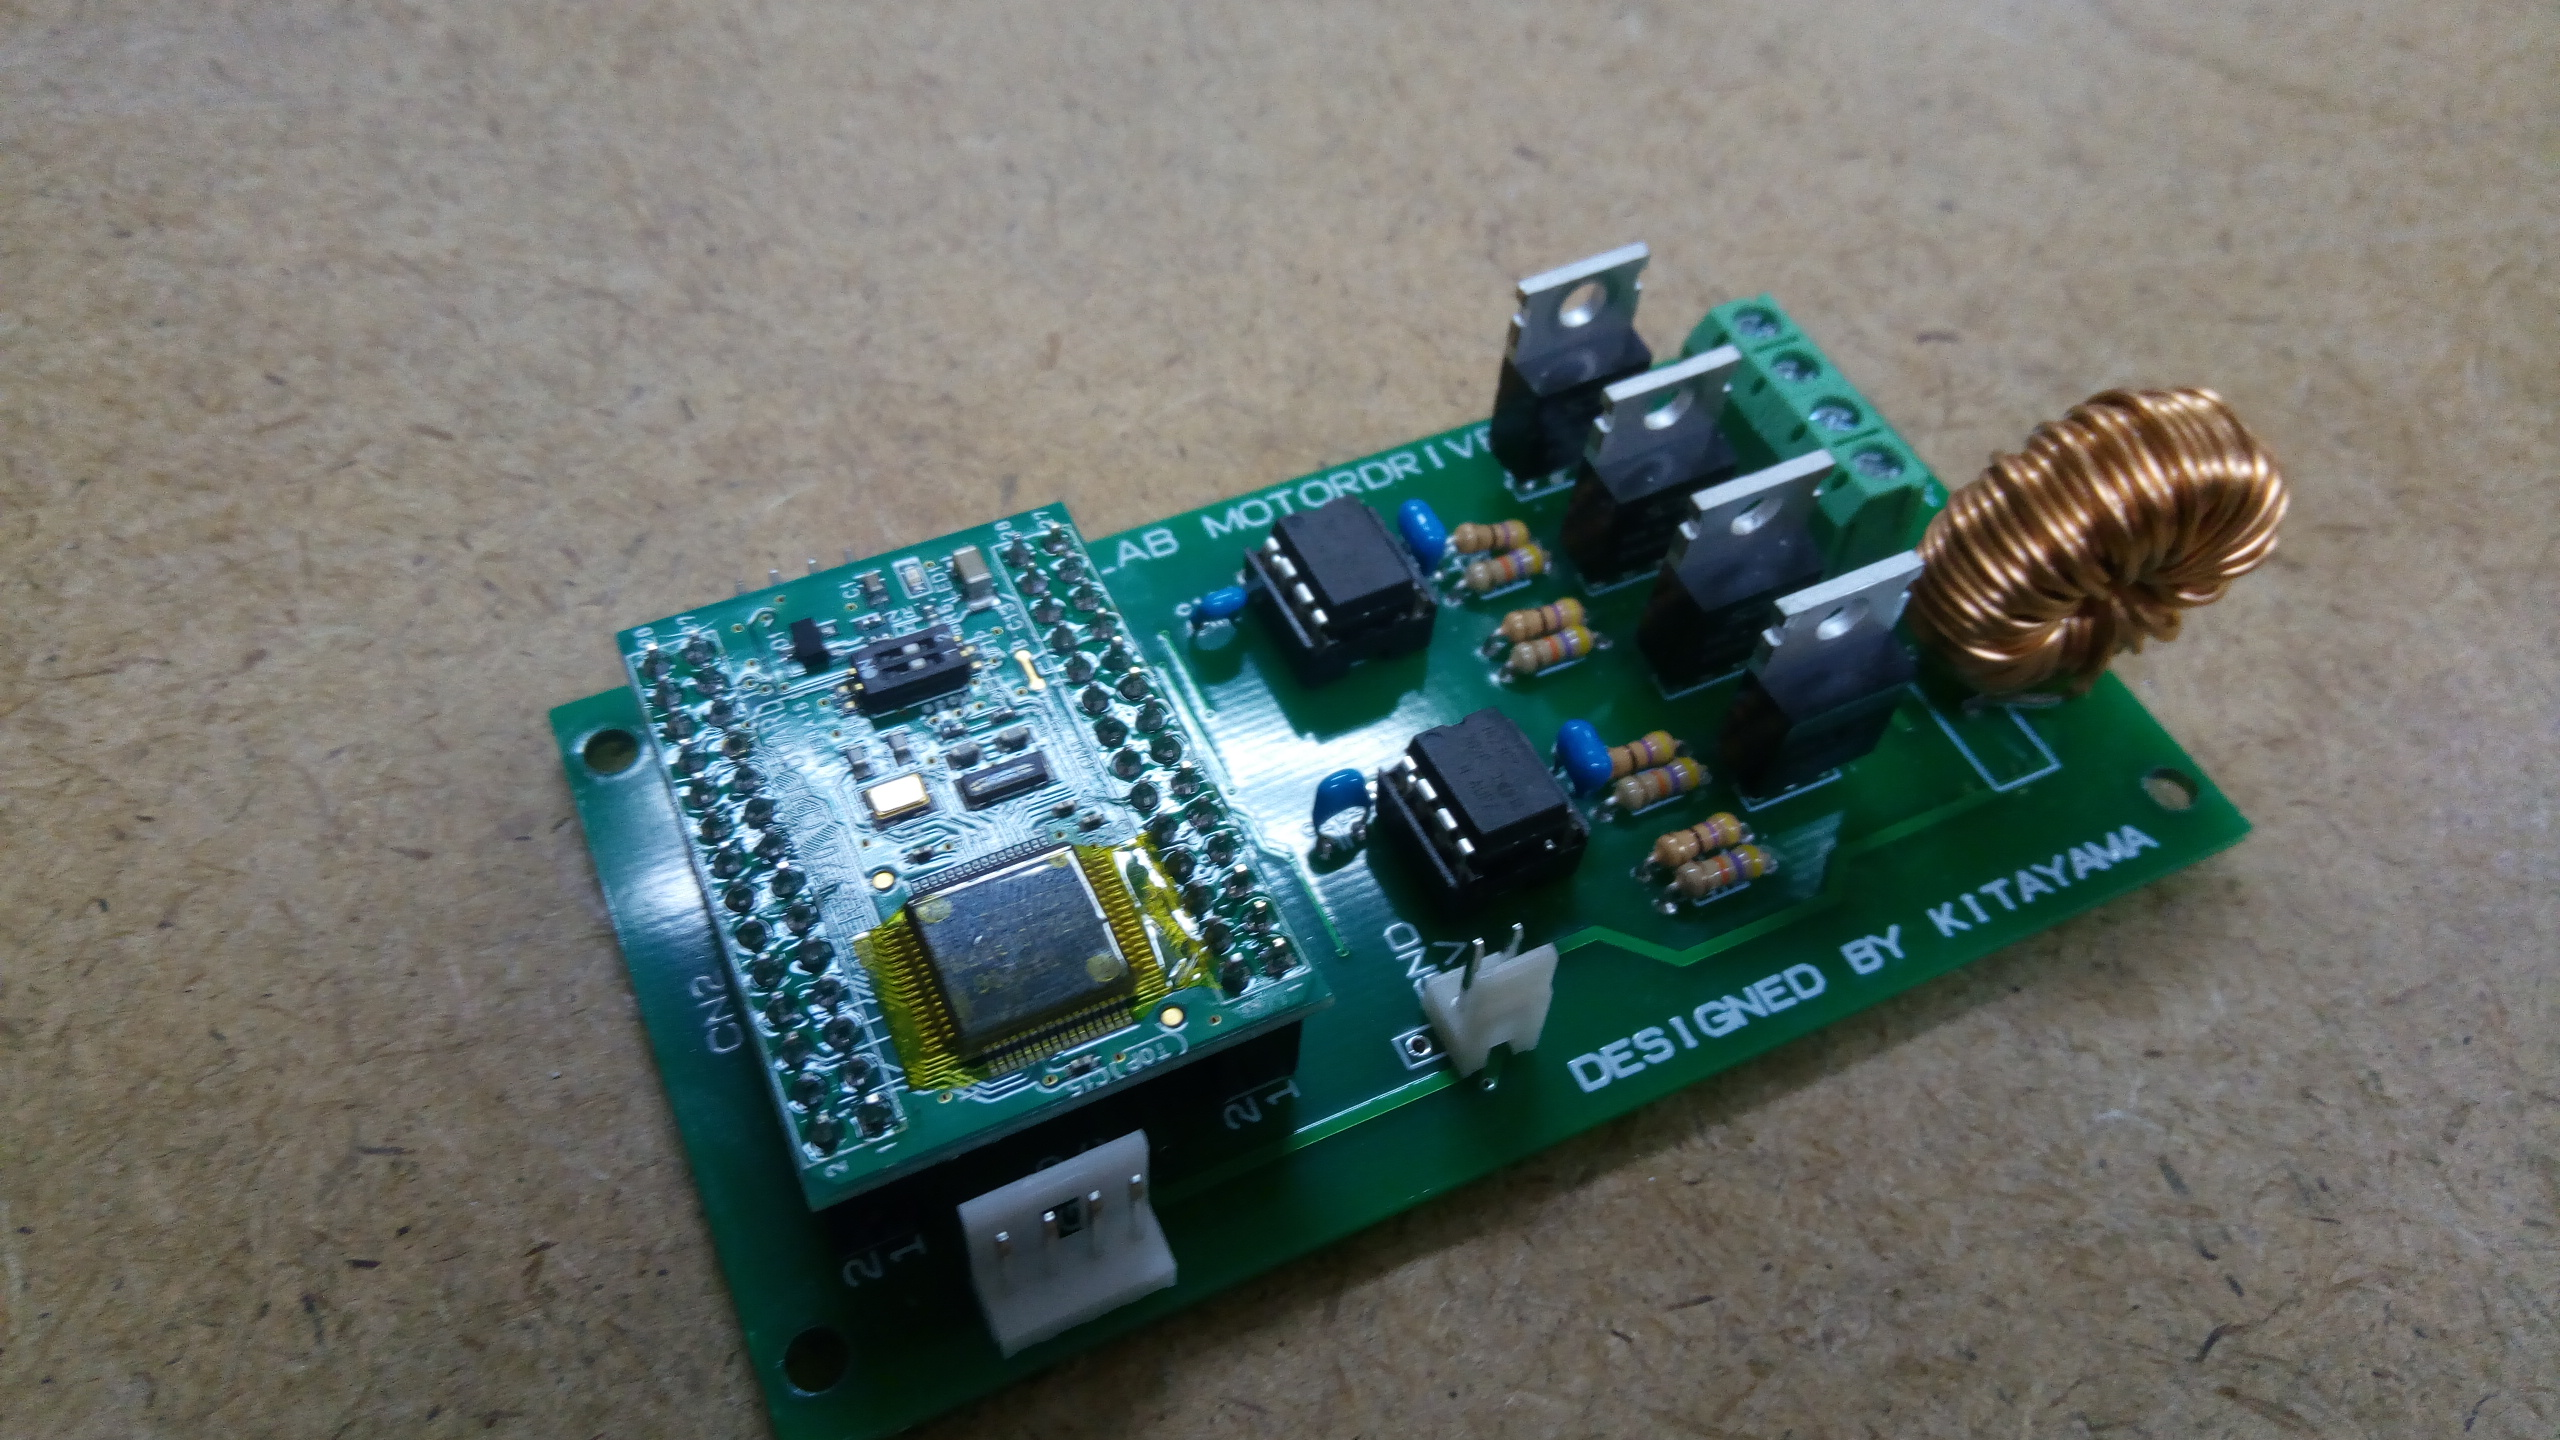
\includegraphics[width=48mm]{driver}
    \end{center}
  \caption{ITOLAB MOTORDRIVER}
 \label{fig:driver}
\end{figure}

\subsection{改善点}
ロボットの動作実験では,急加減速時にパターンの焼損,回生電流によるノイズの発生,
FETトランジスタの高温化,通信エラーなどの問題が発生した.これらを改善するために,
電流制限プログラムの作成,回生ダイオードの取り付け,FETトランジスタにヒートシンクの
取り付け,通信エラー確認用のLEDの取り付けを行った.
改善後のITOLAB MOTORDRIVERを図\ref{fig:shin_driver}に示す.
\begin{figure}[H]
  \begin{center}
    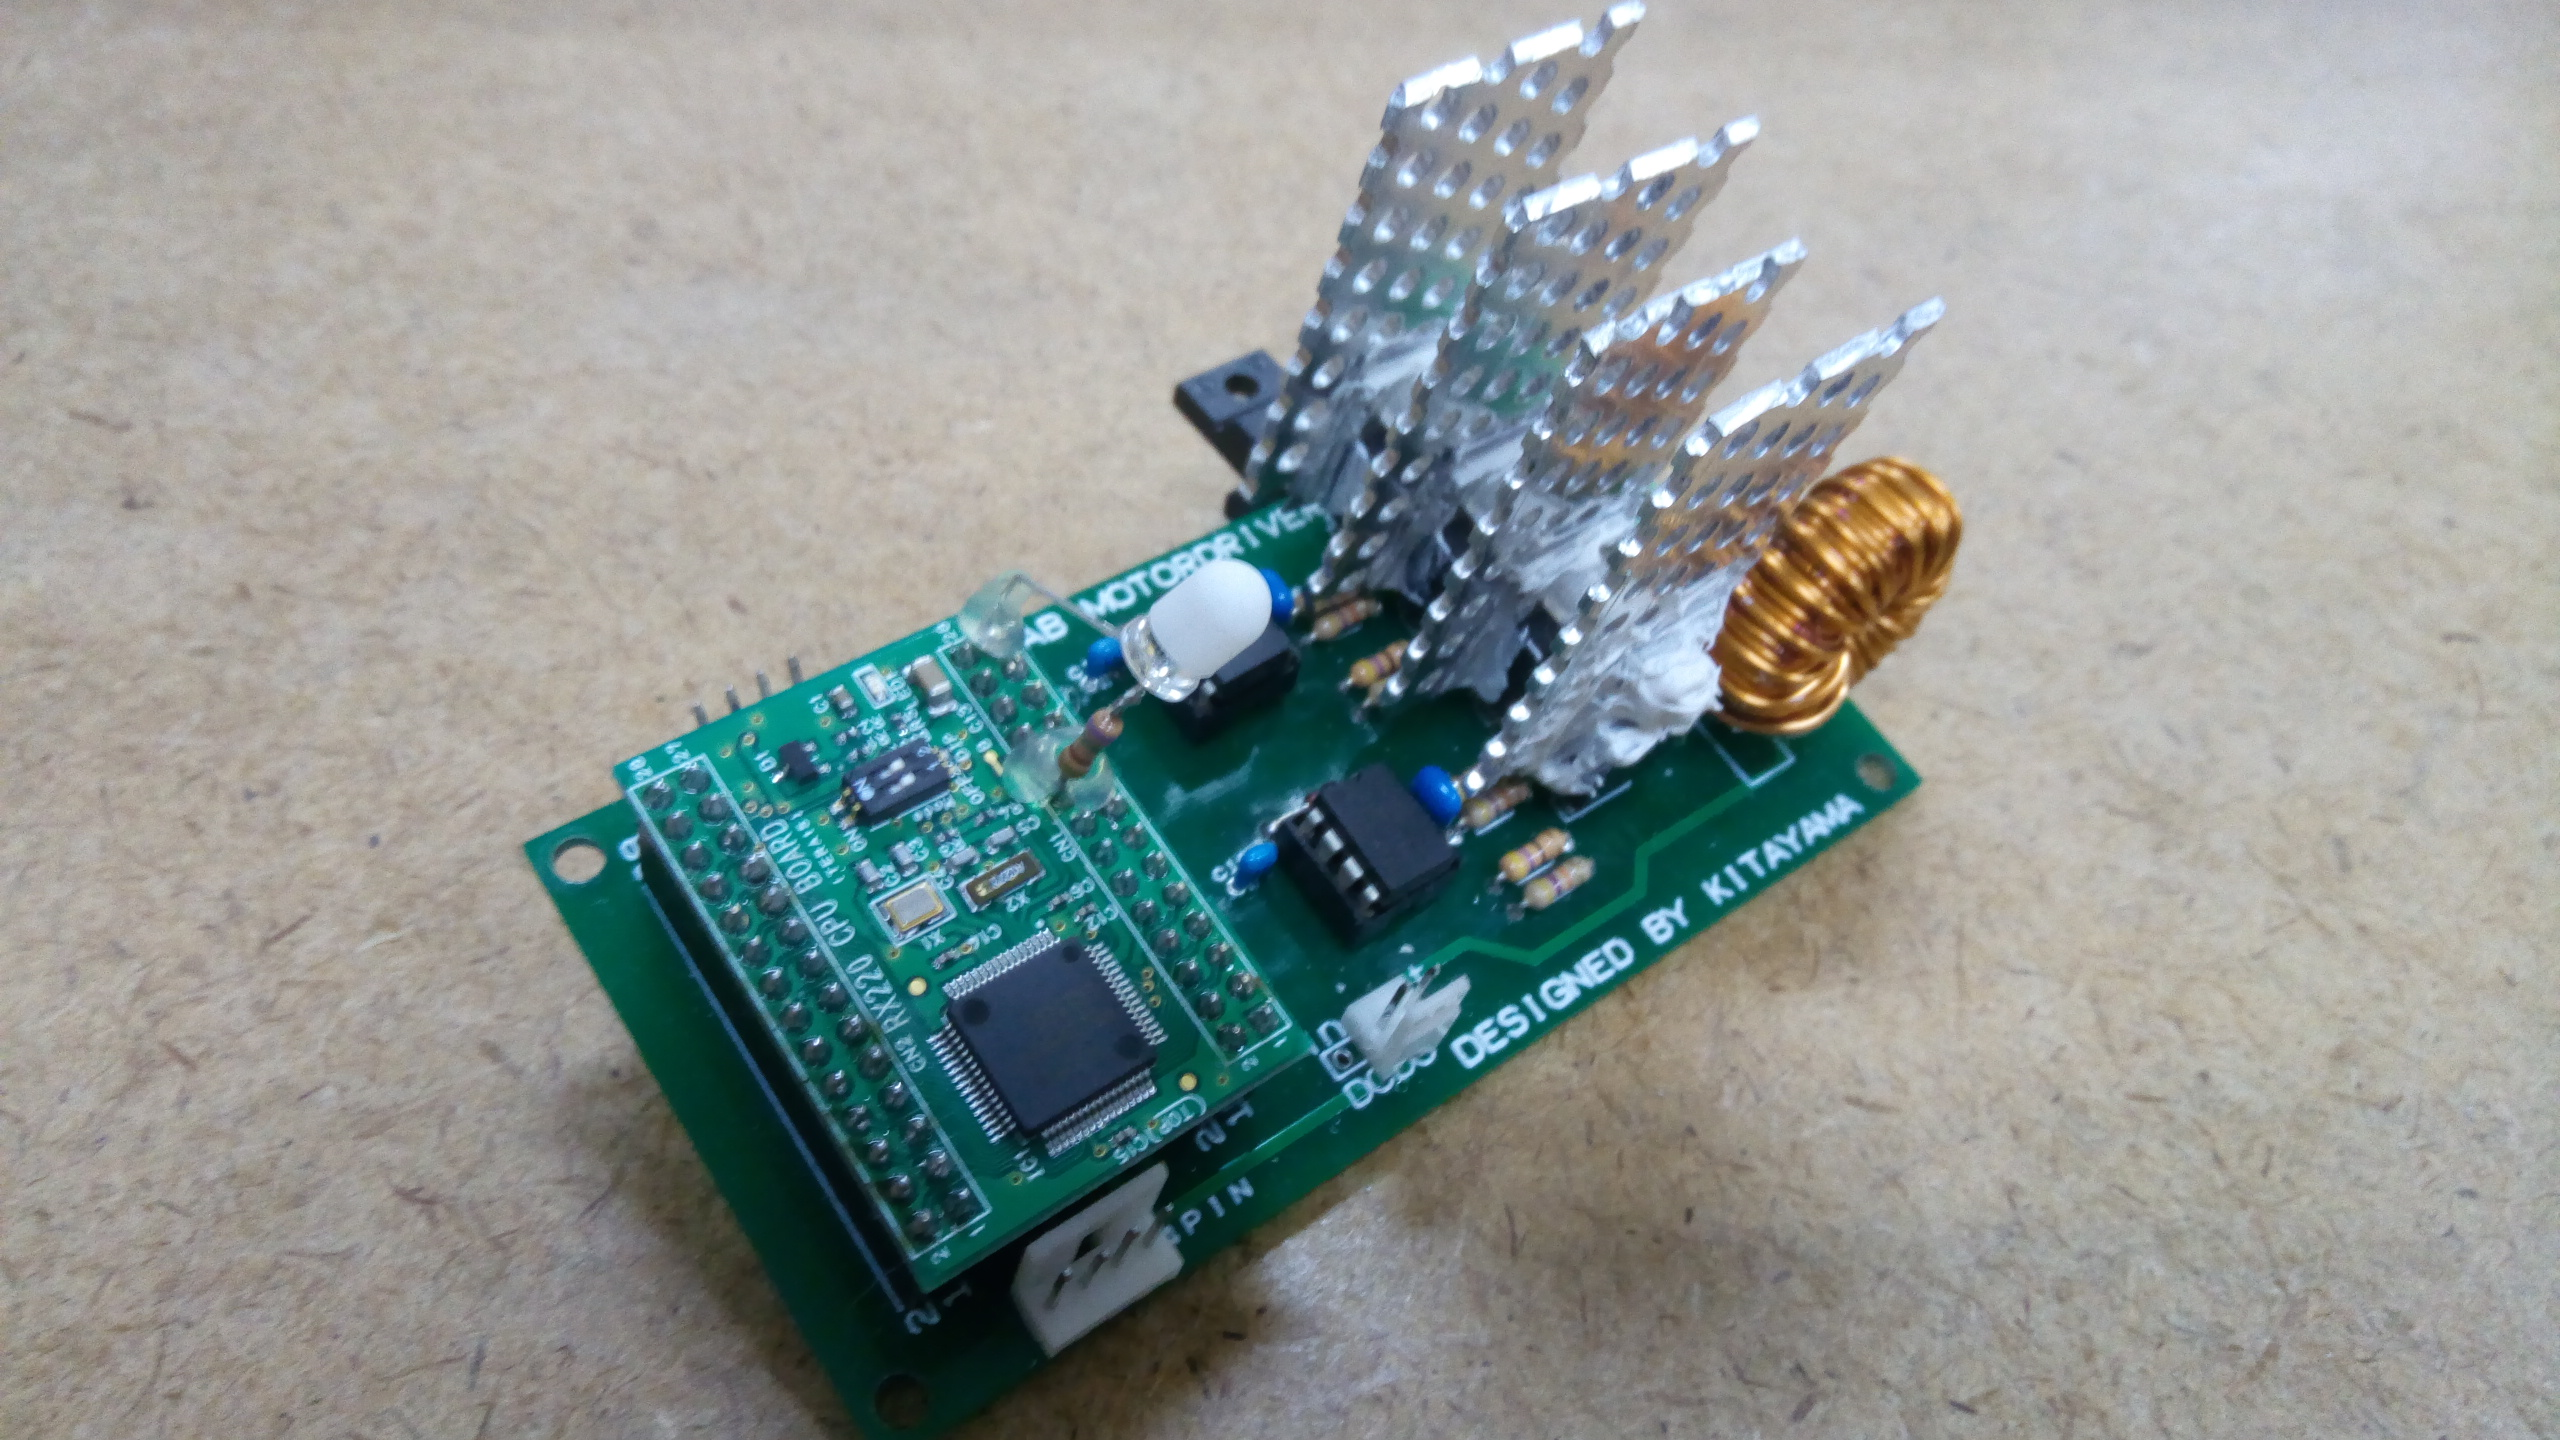
\includegraphics[width=48mm]{shin_driver}
    \end{center}
  \caption{改善後のITOLAB MOTORDRIVER}
 \label{fig:shin_driver}
\end{figure}

\subsection{動作不具合}
回路の発熱防止のための電流制限により,モータ回転数が目標の1114rpmに達せず,
700rpmまでとなった.
また,地区大会時に1台のロボットのモータが動作
しなくなり,また試合後モータドライバの不具合も発見できなかった.

\section{新高出力モータドライバ}
\subsection{要求機能}
先に述べた不具合箇所を修正,改良した高出力モータドライバを製作した.
\begin{itemize}
\item 大電流が流れるパターン幅の拡張,GNDのベタ化
\item FETヒートシンク,回生ダイオードの標準搭載
\item FET用温度センサ,電流センサ,エラー確認用LEDの取り付け
\item 制御用マイコンのリセットスイッチ,汎用スイッチの搭載
\item ノイズの影響を受けやすいRS232通信から,影響を受けにくいRS485通信へ変更
\end{itemize}

\subsection{構成}
新高出力モータドライバのシステムブロック図を図\ref{fig:shisutemu}に示す.
また,新モータドライバの仕様を表\ref{tab:shinshiyou}に示す.
制御用の信号は全てRXマイコンで入出力される.
\begin{figure}[H]
  \begin{center}
    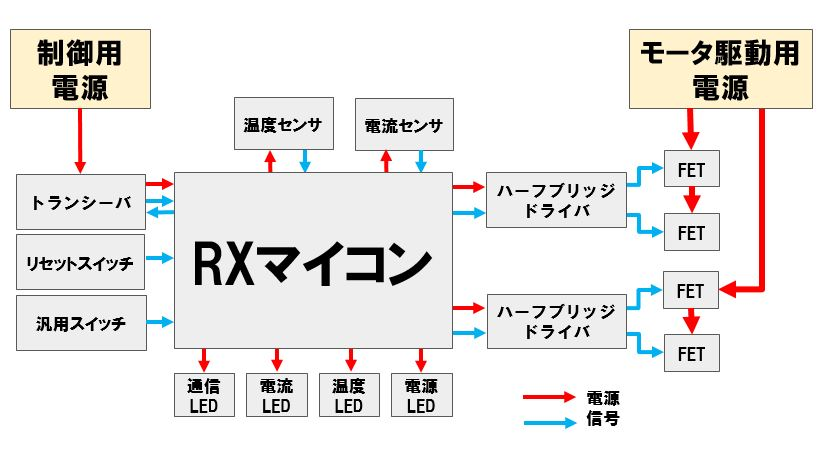
\includegraphics[width=80mm]{shisutemu}
    \end{center}
  \caption{システムブロック図}
 \label{fig:shisutemu}
\end{figure}
\begin{table}[htb]
\centering
\caption{新モータドライバの仕様書}
\begin{tabular}{|c|c|} \hline
使用マイコン&RX220マイコン\\ \hline
シリアル通信&RS485\\ \hline
温度センサ&動作温度 -40~125℃ \\
&動作電圧 3.1~5.5V \\ \hline
電流センサ&動作温度 -40~150℃\\
&作動電圧 3.3~5.5V \\
&検出電圧 0~100A \\ \hline
\end{tabular}
\label{tab:shinshiyou}
\end{table}

\subsection{回路図・アートワーク}
新高出力モータドライバの回路図を図\ref{fig:kairozu}に示す.
回路図とアートワークの作成は,回路図とアートワークが連動しているKiCadを用いた.
回路図は,ITOLAB MOTORDRIVERの回路図を作成した後に,新たに追加する部品を接続した.
アートワークは,大電流の流れるパターン幅を,1.0mmから5.0mmに変更した.
また,裏面はGNDのベタ化を行った.
\begin{figure}[H]
\begin{center}
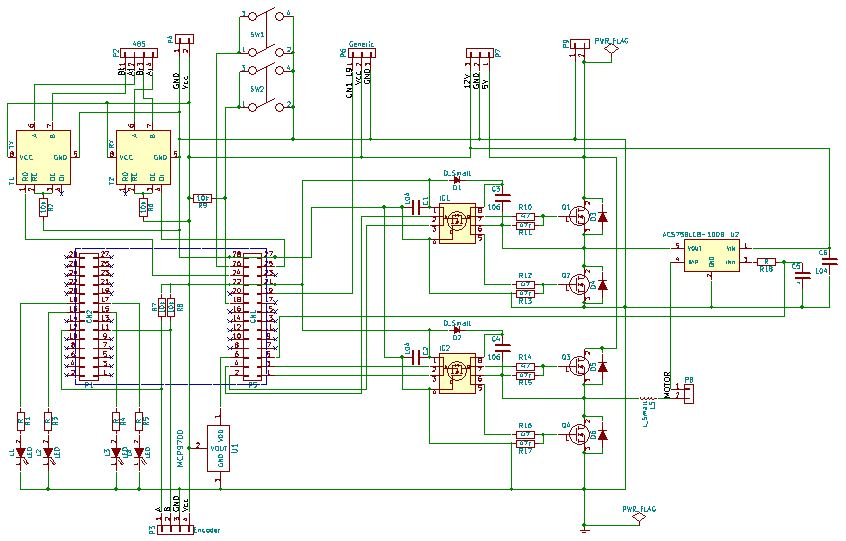
\includegraphics[width=80mm]{kairozu}
\end{center}
\caption{回路図}
\label{fig:kairozu}
\end{figure}

\subsection{完成品}
ロボコン用高出力モータードライバの完成品を図\ref{fig:kankumi}に示す.
プリント基板の製造は,Fusion PCBに依頼した.
\begin{figure}[H]
\begin{center}
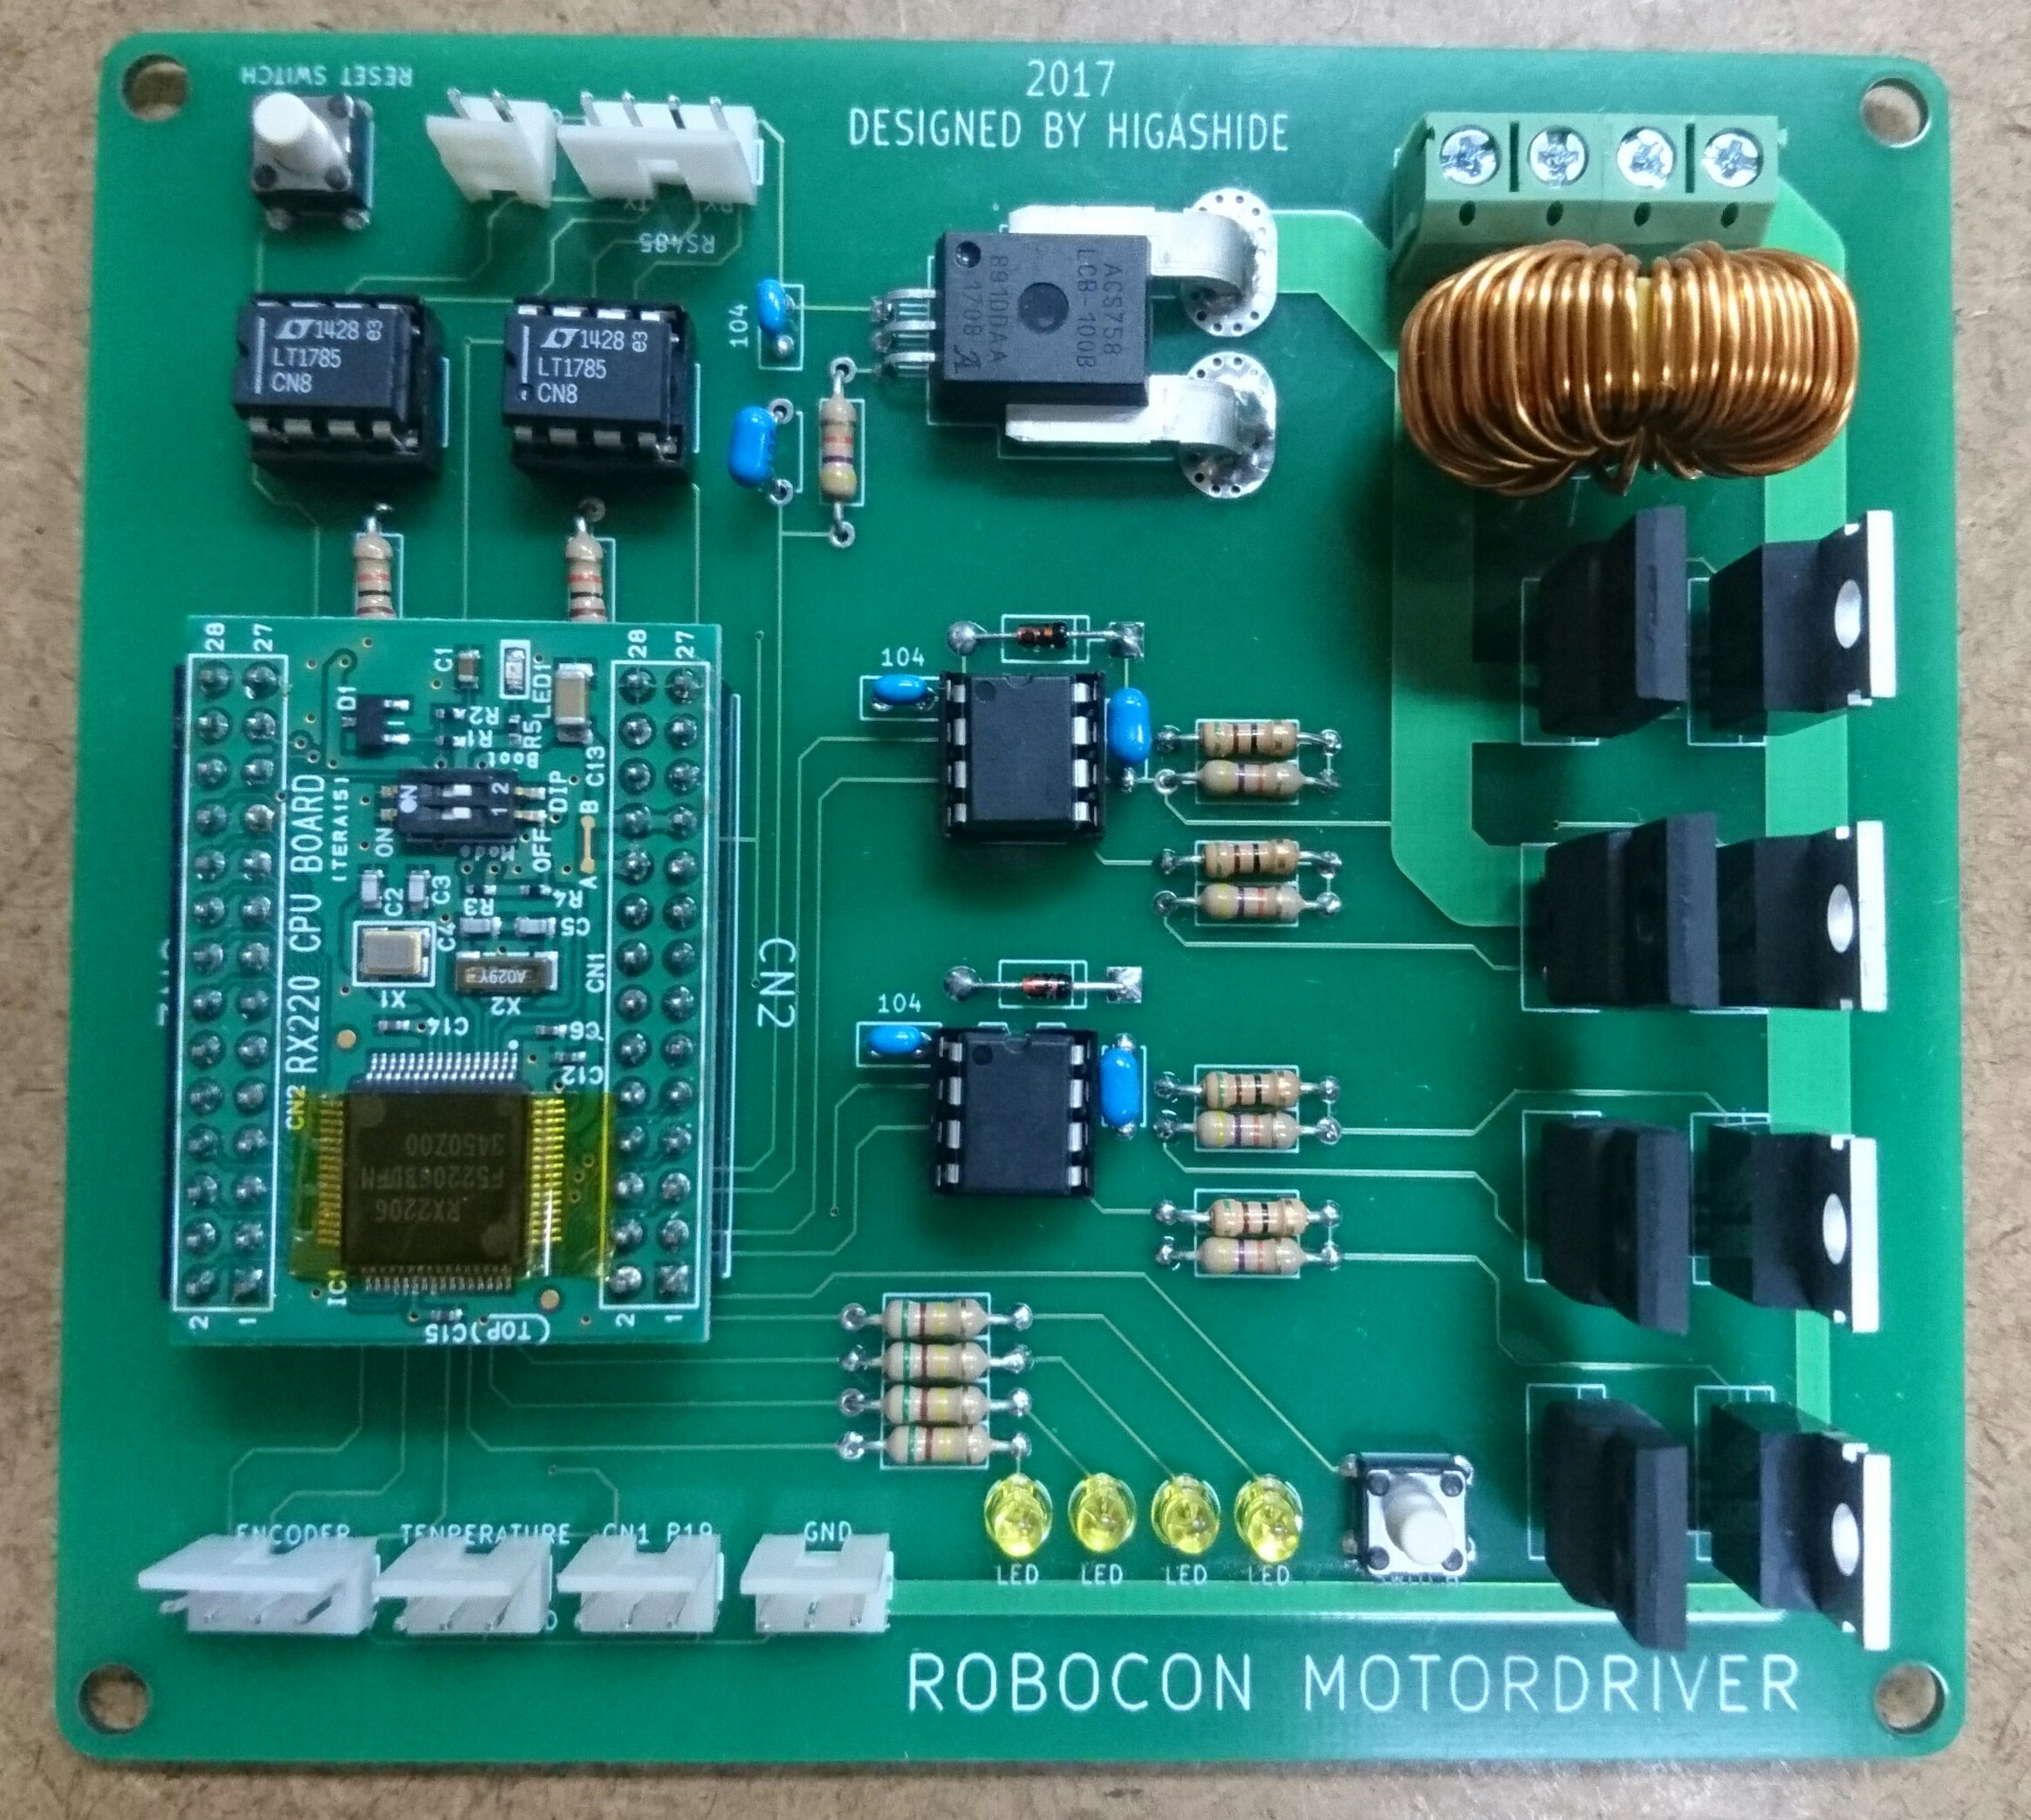
\includegraphics[width=70mm]{kankumi}
\end{center}
\caption{完成品}
\label{fig:kankumi}
\end{figure}

\subsection{動作確認}
リセットスイッチによるRXマイコンのリセット動作,汎用スイッチの動作,汎用LEDの点灯,
RXマイコンからのPWM信号の出力を確認した.
また,モータを時計回り,反時計回りに回転させることができた.

\subsection{今後の課題}
電流センサ,温度センサの検出値の確認,RXマイコンによるシリアル通信の確認が必要である.


\section{おわりに}
既存のドライバを改良することによって,短期間で高出力モータドライバの設計,作製を
行うことができた.
また,無料配布されているKiCadを使用することによって,回路図,アートワークも短期間で
作成することができた.

% 参考文献
\begin{thebibliography}{8}
\bibitem{hon}寺前裕司,1人で始めるプリント基板作り[完全フリーKicad付き],CQ出版株式会社,2014/7/1
\bibitem{ob} KiCADで基本設計,\url{http://www.kicad.xyz/}
\bibitem{sei} KiCad で雑に基板を作る チュートリアル,\url{https://www.slideshare.net/soburi/kicad-53622272}
\end{thebibliography}
\end{document}



